 %%%%%%%%% %%%%%%%%% %%%%%%%%% %%%%%%%%% %%%%%%%%% %%%%%%%%% %%%%%%%%%
\chapter{Metodi}
\label{cap:methods}

\section{Force-clamp}


In figura \ref{fig:setup} è mostrato uno schema integrale
dell'apparato realizzato.
Le componenti principali sono descritte nella sezione \ref{sec:setup}.
Successivamente, nella sezione \ref{sec:stabilization} è descritto il
sistema di stabilizzazione meccanica introdotto per compensare lo
spostamento
del campione dovuto a deriva termica e oscillazioni acustiche.
Nella sezione \ref{sec:calibration} è descritta nel dettaglio la
procedura usata per la calibrazione dei parametri delle trappole
ottiche.

L'esperimento tipico utilizzato per studiare l'interazione tra una
proteina e un microfilamento di actina consiste in un saggio a tre
sfere, o \textit{3-beads assay}. I dettagli per la realizzazione di
questo esperimento sono illustrati nella sezione \ref{sec:3beads}.

\section{Apparato sperimentale}
\label{sec:setup}

L'apparato sperimentale è stato realizzato presso i laboratori del
LENS, sulla base dell'apparato utilizzato in precedenza dal di
Biofisica di Singola Molecola per lo studio delle interazioni tra
miosina e filamenti di actina e repressori della trascrizione
e filamenti di DNA.

L'apparto si compone di N parti principali:
\begin{description}
    \item[Pinzette ottiche:] Una coppia di fasci gaussiani a \SI{1064}{\nm}, ottenuti da un laser a stato solido, 
\end{description}



\begin{sidewaysfigure}
    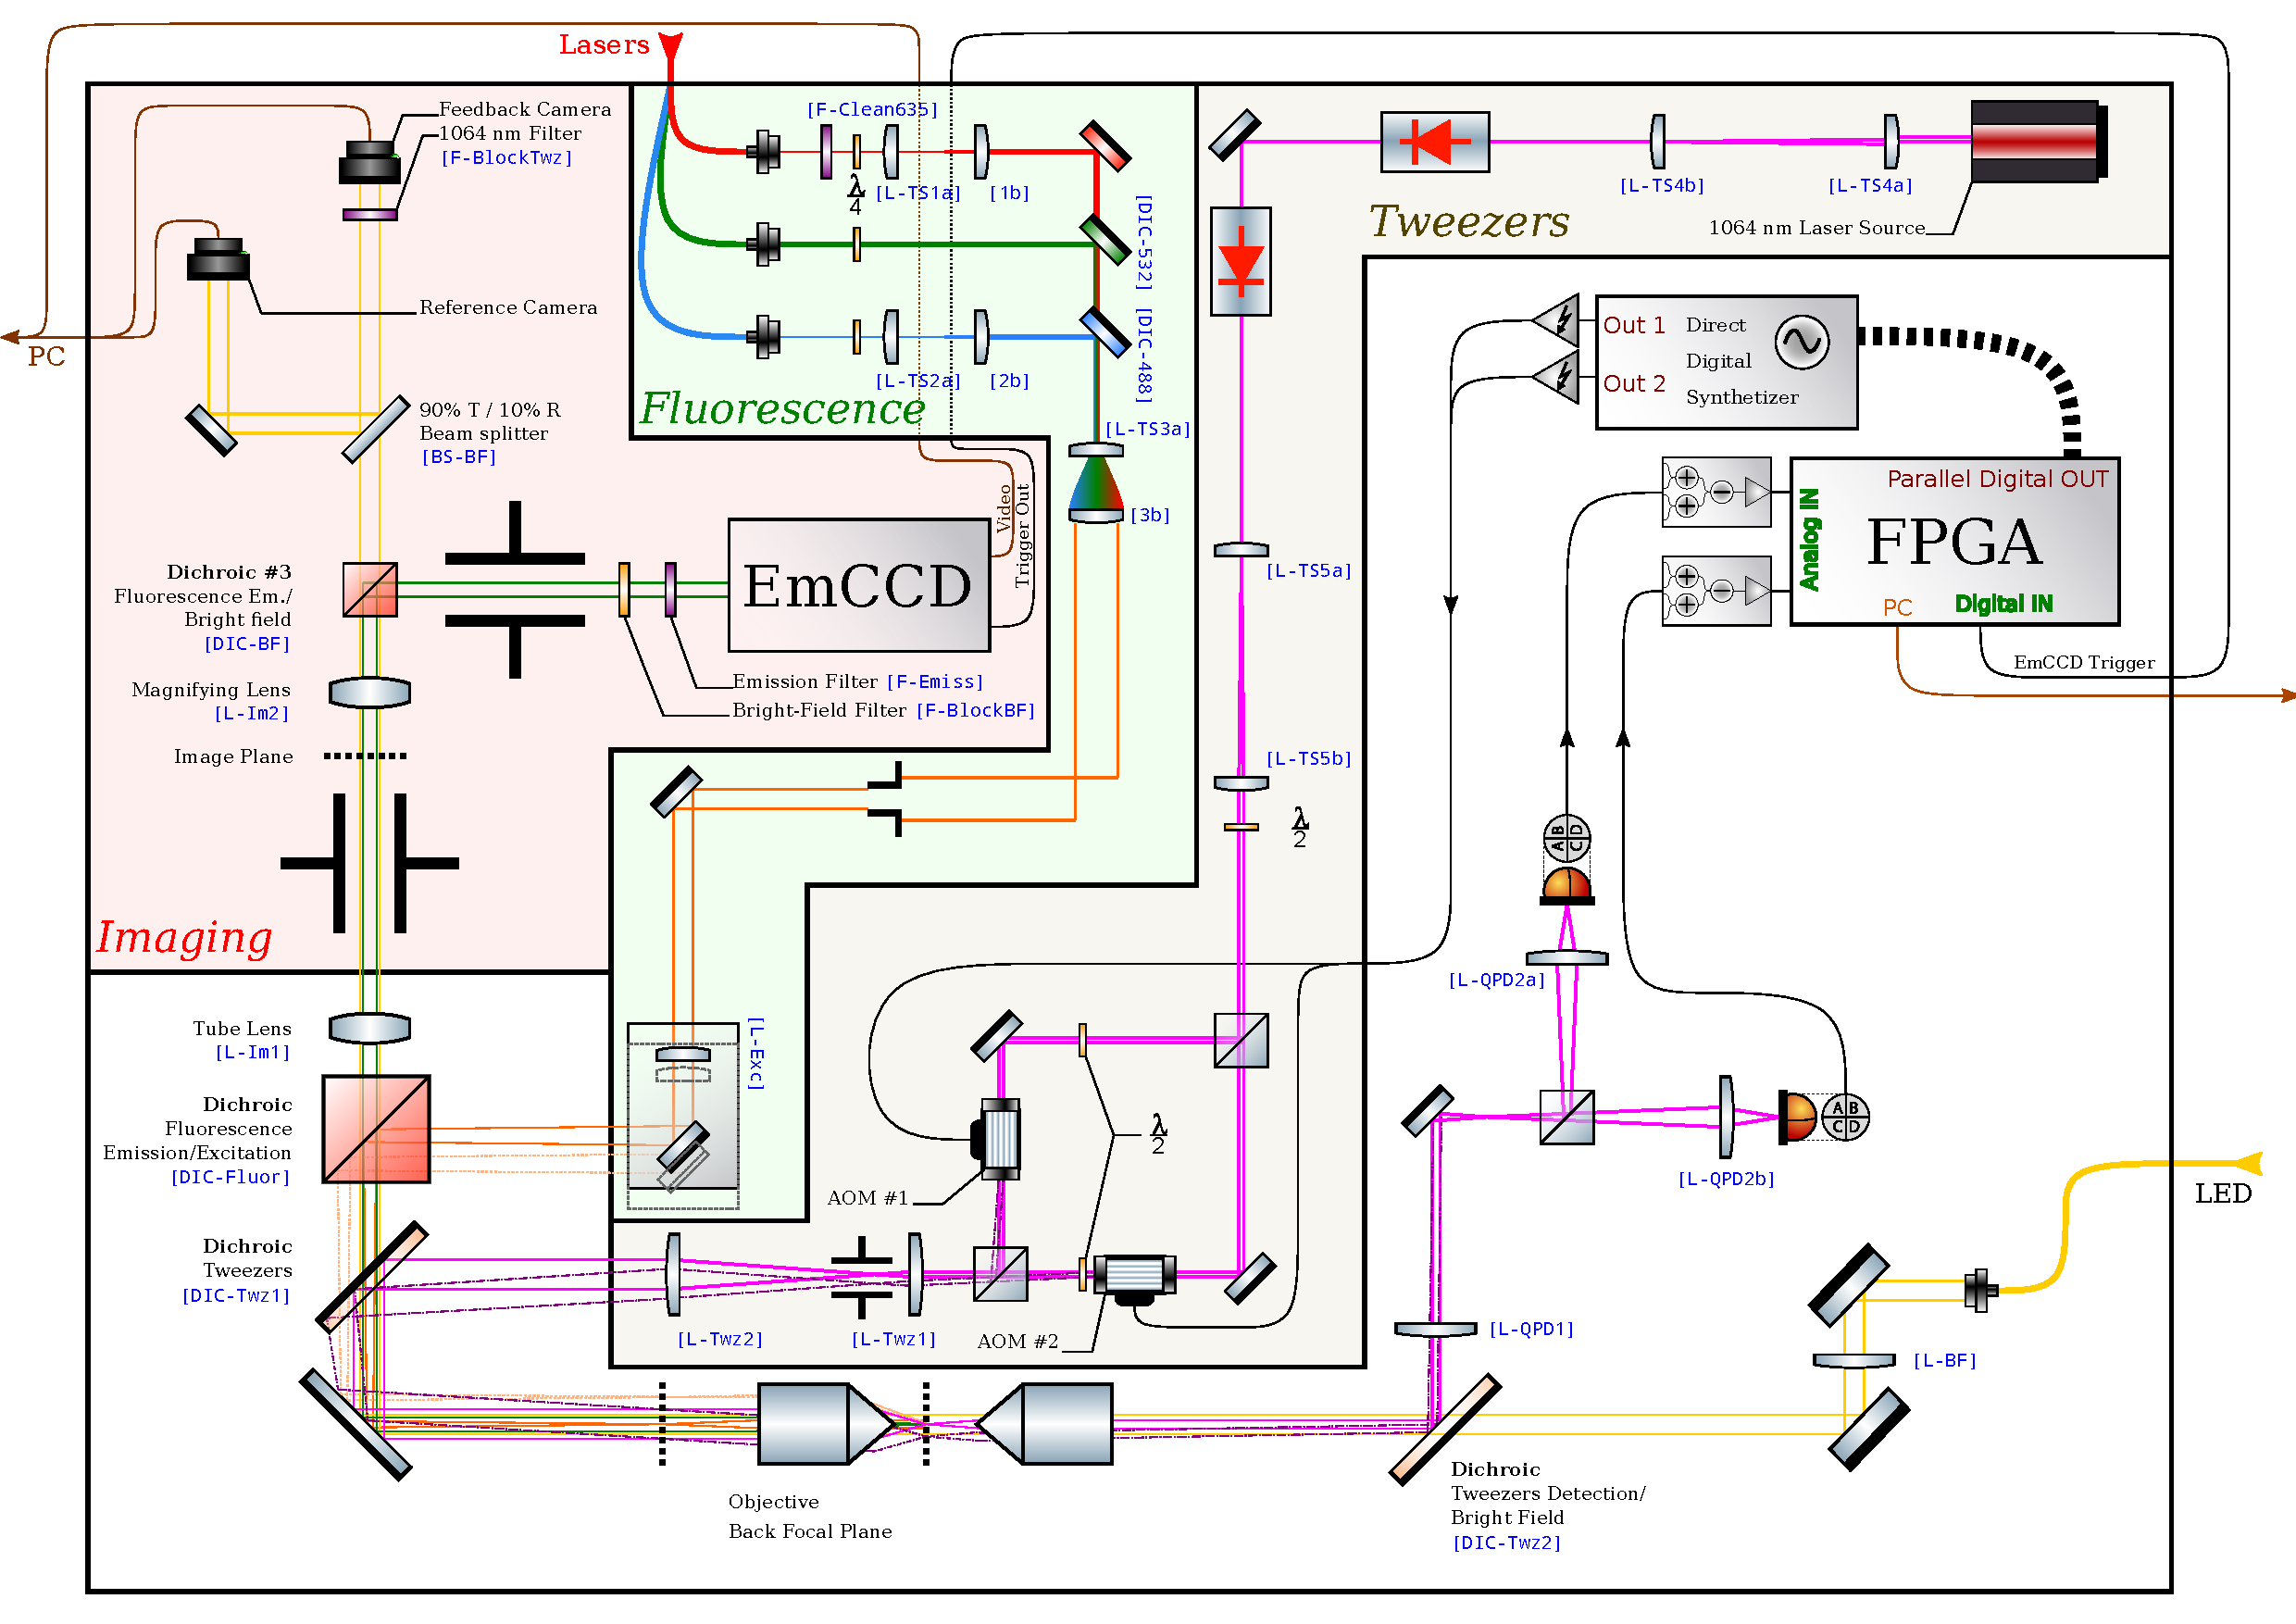
\includegraphics[width=1.0\linewidth]{images/Setup.pdf}
    \caption{Caption}
    \label{fig:setup}
\end{sidewaysfigure}

\begin{sidewaystable}
    \centering
    \begin{tabular}{>{\tt}l l l >{\it}l l}
    \toprule
         Code & Type & Usage & Parameters & Product ID\\
    \midrule
    \multicolumn{5}{l}{\it Fluorescence Excitation Path}\\
        F-Clean635
            & Bandpass Filter
            & \SI{635}{\nm} laser clean-up
            & $\lambda_{centr}: \SI{640}{\nm},
              bw: \SI{14}{\nm}$
            & FF01-640/14-25\\
        L-TS1a
            & Plano-Convex Spherical Lens
            & Telescope for \SI{635}{\nm} laser
            & f: \SI{0}{\mm}
            & \\
        L-TS1b
            & & 
            & f: \SI{0}{\mm}
            & \\
        L-TS2a
            & 
            & Telescope for \SI{488}{\nm} laser
            & f: \SI{0}{\mm}
            & \\
        L-TS2b
            & & 
            & f: \SI{0}{\mm}
            & \\
        DIC-532
            & Single-edge Dichroic Filter
            & Excitation beam multiplexing
            & $\lambda_{edge}: \SI{532}{\nm}$
            & Di02-R532-25-D\\
        DIC-488
            & &
            & $\lambda_{edge}: \SI{488}{\nm}$
            & Di02-R488-25-D\\
        L-TS3a
            & Achromatic Doublet
            & Telescope for comb. ex. lasers
            & f: \SI{0}{\mm}
            & \\
        L-TS3b
            & & 
            & f: \SI{0}{\mm}
            & \\
        L-Exc
            &
            & Excitation beam focusing
            & f: \SI{0}{\mm} 
            & \\
        DIC-Fluor
            & Quad-edge Dichroic Filter
            & Excitation/Emission separation
            & $\lambda_{edge}: \SIlist{405;488;532;635}{\nm}$
            & Di03-R405/488/532/635-t1 \\
    \multicolumn{5}{l}{\it Tweezers Path}\\
        L-TS4a
            & Plano-Convex Spherical Lens
            & Telescope matching isolator size
            & f: \SI{0}{\mm}
            & \\
        L-TS4b
            & & 
            & f: \SI{0}{\mm}
            & \\
        L-TS5a
            & Plano-Convex Spherical Lens
            & Telescope after isolator
            & f: \SI{0}{\mm}
            & \\
        L-TS5b
            & & 
            & f: \SI{0}{\mm}
            & \\
        L-Twz1
            & Plano-Convex Spherical Lens
            & Telescope after isolator
            & f: \SI{0}{\mm}
            & \\
        L-Twz2  
            & & 
            & f: \SI{0}{\mm}
            & \\
        DIC-Twz1
            & Single-edge Dichroic Filter
            & Tweezer beam insertion
            & $\lambda_{edge}: \SI{1064}{\nm}$
            & \\
    \multicolumn{5}{l}{\it Imaging Path}\\
        L-Im1  
            & Tube Lens
            & Tube Lens
            & f: \SI{0}{\mm}
            & \\
        L-Im2  
            & Imaging Lens
            & Imaging Lens
            & f: \SI{0}{\mm}
            & \\
        DIC-BF
            & Single-edge Dichroic Filter
            & Fluorescence/Brightfield demux
            & $\lambda_{edge}: \SI{705}{\nm}$
            & FF705-Di01-25x36\\
        F-BlockBF
            & Shortpass Filter
            & Residual brightfield suppression
            & $\lambda_{cut}: \SI{700}{\nm}$
            & FESH0700\\
        F-Emiss
            & Quad-band bandpass Filter
            & Fluorophore emission filtering
            & $\lambda_{centr}: \SIlist{446;510;581;703}{\nm}$
            & FF01-446/510/581/703\\
        F-BlockTwz
            & Bandstop filter
            & Fluorophore emission filtering
            & $\lambda_{centr}: \SIlist{446;510;581;703}{\nm}$
            & FF01-446/510/581/703\\
     \end{tabular}
     \caption{Caption}
     \label{tab:my_label}
 \end{sidewaystable}
 
 
 \section{Stabilizzazione meccanica}
 \label{sec:stabilization}